% -------------------------------------------------------------------------------------------------
% DensityMapNet architecture (src/models/density_map.py).
%
% Standalone TikZ diagram: compile with
%     pdflatex density_map_architecture.tex
% (or latexmk -pdf). Only the standard TikZ libraries are used, so any TeX Live/MiKTeX works.
%
% Shapes are written as (batch, channels, height, width); H = preset["density"]["decoder_hidden"] = 64,
% grid = 32, sigma = 0.06. The spatial size on the arrows is the output of each upsampling step for a
% 4x4 seed: (4-1)*2 - 2 + 4 = 8 -> 16 -> 32.
% -------------------------------------------------------------------------------------------------
\documentclass[tikz,border=8pt]{standalone}
\usepackage[T1]{fontenc}
\usetikzlibrary{arrows.meta, positioning, fit, backgrounds, calc, shapes.geometric}

\definecolor{enc}{HTML}{2C7FB8}
\definecolor{dec}{HTML}{31A354}
\definecolor{head}{HTML}{D95F0E}
\definecolor{aux}{HTML}{756BB1}

\begin{document}
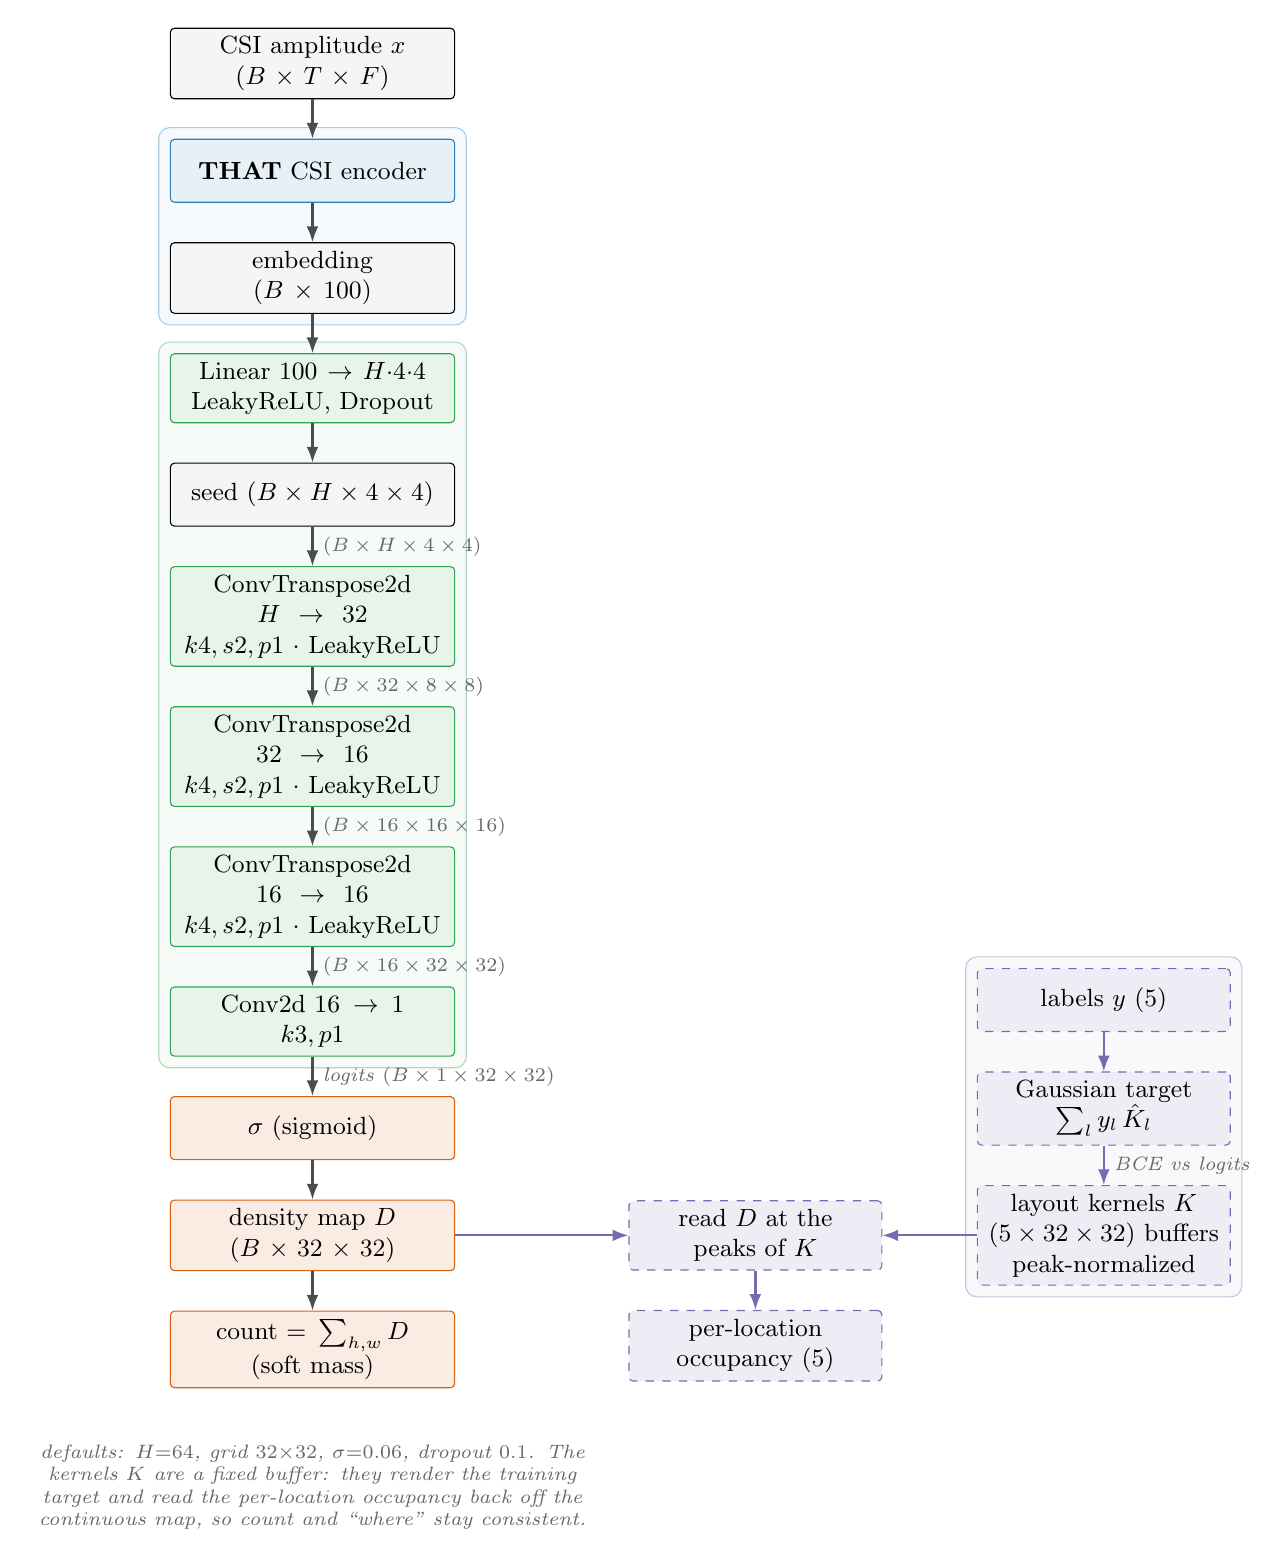
\begin{tikzpicture}[
    node distance = 5mm and 12mm,
    > = {Latex[length=2mm]},
    box/.style   = {draw, rounded corners=1.5pt, align=center, font=\small,
                    inner sep=3pt, minimum height=8mm, text width=34mm},
    tensor/.style = {box, fill=black!4},
    encbox/.style = {box, fill=enc!12,  draw=enc},
    decbox/.style = {box, fill=dec!12,  draw=dec},
    headbox/.style= {box, fill=head!12, draw=head},
    auxbox/.style = {box, fill=aux!12,  draw=aux, dashed, text width=30mm},
    flow/.style   = {->, thick, draw=black!70},
    auxflow/.style= {->, thick, draw=aux},
    note/.style   = {font=\scriptsize\itshape, text=black!60},
]

% --------------------------------------------- encoder -------------------------------------------
\node[tensor]  (x)    {CSI amplitude $x$\\$(B\times T\times F)$};
\node[encbox, below=of x]    (that) {\textbf{THAT} CSI encoder};
\node[tensor, below=of that] (emb)  {embedding\\$(B\times 100)$};
\node[decbox, below=of emb]  (fc)   {Linear $100\to H{\cdot}4{\cdot}4$\\LeakyReLU, Dropout};
\node[tensor, below=of fc]   (seed) {seed $(B\times H\times 4\times 4)$};

% --------------------------------------------- decoder -------------------------------------------
\node[decbox, below=of seed] (c1) {ConvTranspose2d $H\to32$\\$k4,s2,p1$ $\cdot$ LeakyReLU};
\node[decbox, below=of c1]   (c2) {ConvTranspose2d $32\to16$\\$k4,s2,p1$ $\cdot$ LeakyReLU};
\node[decbox, below=of c2]   (c3) {ConvTranspose2d $16\to16$\\$k4,s2,p1$ $\cdot$ LeakyReLU};
\node[decbox, below=of c3]   (cv) {Conv2d $16\to1$\\$k3,p1$};
\node[headbox, below=of cv]  (sig){$\sigma$ (sigmoid)};

% ---------------------------------------------- heads --------------------------------------------
\node[headbox, below=of sig] (dens)  {density map $D$\\$(B\times32\times32)$};
\node[headbox, below=of dens](cnt)   {count $=\sum_{h,w} D$\\(soft mass)};

% ----------------------------------------- location readout ---------------------------------------
\node[auxbox, right=22mm of dens] (read) {read $D$ at the peaks of $K$};
\node[auxbox, below=of read]      (occ)  {per-location occupancy $(5)$};
\node[auxbox, right=of read]      (kern) {layout kernels $K$\\$(5\times32\times32)$ buffers\\peak-normalized};

% ------------------------------------------- training ---------------------------------------------
\node[auxbox, above=of kern]  (targ) {Gaussian target\\$\sum_l y_l\,\hat{K}_l$};
\node[auxbox, above=of targ]  (lab)  {labels $y$ $(5)$};

% --------------------------------------------- arrows ---------------------------------------------
\draw[flow] (x) -- (that);
\draw[flow] (that) -- (emb);
\draw[flow] (emb) -- (fc);
\draw[flow] (fc) -- (seed);
\draw[flow] (seed) -- node[right, note] {$(B\times H\times4\times4)$} (c1);
\draw[flow] (c1) -- node[right, note] {$(B\times32\times8\times8)$} (c2);
\draw[flow] (c2) -- node[right, note] {$(B\times16\times16\times16)$} (c3);
\draw[flow] (c3) -- node[right, note] {$(B\times16\times32\times32)$} (cv);
\draw[flow] (cv) -- node[right, note] {logits $(B\times1\times32\times32)$} (sig);
\draw[flow] (sig) -- (dens);
\draw[flow] (dens) -- (cnt);

\draw[auxflow] (dens) -- (read);
\draw[auxflow] (kern) -- (read);
\draw[auxflow] (read) -- (occ);
\draw[auxflow] (lab) -- (targ);
\draw[auxflow] (targ) -- node[right, note] {BCE vs logits} (kern);

% --------------------------------------------- groups ---------------------------------------------
\begin{scope}[on background layer]
    \node[draw=enc!40,  fill=enc!4,  rounded corners, fit=(that)(emb), inner sep=4pt] {};
    \node[draw=dec!40,  fill=dec!4,  rounded corners, fit=(fc)(cv),     inner sep=4pt] {};
    \node[draw=aux!40,  fill=aux!4,  rounded corners, fit=(kern)(targ)(lab), inner sep=4pt] {};
\end{scope}

% --------------------------------------------- caption --------------------------------------------
\node[note, below=6mm of cnt, text width=70mm, align=center]
    {defaults: $H{=}64$, grid $32{\times}32$, $\sigma{=}0.06$, dropout $0.1$.
     The kernels $K$ are a fixed buffer: they render the training target and read the
     per-location occupancy back off the continuous map, so count and ``where'' stay consistent.};

\end{tikzpicture}
\end{document}
